\documentclass[12pt,a4paper]{report}
\usepackage[utf8]{inputenc}
\usepackage{amsfonts}
\usepackage{setspace}
\usepackage{graphicx}
\usepackage{array}
\usepackage{fancyhdr}
\usepackage[bottom=3cm]{geometry}
\usepackage{ragged2e}
\usepackage{color}
\usepackage{tabularx}
\usepackage[backend=biber, sorting=none, style=ieee]{biblatex}
\usepackage{color}
\usepackage{float}

\addbibresource{reference.bib} 
\geometry{
a4paper,
total={210mm,297mm},
left=1.0in,
right=0.85in,
top=0.65in,
bottom=0.65in,
}
\begin{document}
\pagestyle{empty}
\begin{center}



  \large \textbf{Submission of Project Report}
  \par
  \textbf{on}
  \par
  \vspace{15pt}
  {\Large \textbf{CLOUD-BASED SMART MONITORING SYSTEM FOR BABY HEALTH AND SAFETY}}
  \par
  \vspace{12pt}
  \par
  \vspace{12pt}
  \par
  \textit{\textbf{Submitted in fulfillment of the requirements for}}
  \par
  \vspace{18pt}
  {\Large \textbf{IUCEE Annual Student Forum 2025}}
  \par
  \vspace{24pt}
  \textit{\textbf{Submitted by}}
  \vspace{8pt}

  \begin{center}
    \begin{tabular}{l@{\hspace{2cm}}r}
      \textbf{\large Aaron Tauro}       & \textbf{4SO21CS002} \\
      \textbf{\large Abhik L Salian}    & \textbf{4SO21CS004} \\
      \textbf{\large Akhil Shetty M}    & \textbf{4SO21CS013} \\
      \textbf{\large H Karthik P Nayak} & \textbf{4SO21CS058} \\
      \textbf{\large Nishayne E Vaz}    & \textbf{4SO20CS099} \\
    \end{tabular}
  \end{center}
  % \begin{center}
  %     \textbf{\large Aaron Tauro}\\
  %     \textbf{\large Abhik L Salian} \\
  %     \textbf{\large Akhil Shetty M}  \\
  %     \textbf{\large H Karthik P Nayak}\\
  %     \textbf{\large Nishayne C Vaz} \\
  % \end{center}

  \vspace{20pt}
  \textit{\textbf{Under the Guidance of}}
  \par
  \vspace{6pt}
  \textbf{Dr Sridevi Saralaya}
  \par
  \vspace{2pt}
  \normalsize { Professor and HOD, Department of CSE }
  \par
  \begin{figure}[hbtp]
    \centering
    
\includegraphics[scale=0.6]{./pic/sjeclogo}
  \end{figure}
  % \large \textbf{DEPT. OF COMPUTER SCIENCE AND ENGINEERING}
  \par \Large \textbf{ST JOSEPH ENGINEERING COLLEGE}
  \par
  \textbf{An Autonomous Institution}
  \par
  {\large{(Affiliated to VTU Belagavi, Recognized by AICTE)}}
  \par
  \vspace{3pt}
  {\large \textbf{Vamanjoor, Mangaluru - 575028, Karnataka}}
  \par
  \vspace{12pt}
  % {\Large \textbf{2024-25}}
\end{center}

\newpage
\pagestyle{plain}
\setstretch{1.2}
\pagenumbering{roman}
\renewcommand{\contentsname}{\centering Table of Contents}
\tableofcontents
\newpage

\listoffigures







%%%%%%%%%%%%%%%%%%%%% Headders and Footers %%%%%%%%%%%%%%%
\setlength{\textheight}{0.98\textheight} % Adjust to leave space above the footer
\setlength{\headheight}{30pt} % Increase space for the header
\setlength{\footskip}{30pt} % Adjust space for the footer
\fancyhf{} % clear header and footer
\fancyhead[L]{Cloud-Based Smart Monitoring System for Baby Health and Safety} % header centered
\fancyhead[R]{Chapter \thechapter} % header centered
\fancyfoot[L]{St. Joseph Engineering College, Mangaluru} % footer centered
\fancyfoot[R]{\thepage} % page number on the right
\renewcommand{\headrule}{%
  {\color[RGB]{0, 0, 0}\hrule width\headwidth height 2pt} % Top line
  \vspace{0.07\baselineskip}% Add space between lines
  {\color[RGB]{0, 0, 0}\hrule width\headwidth height 0.5pt} % Bottom line
}
\renewcommand{\footrule}{%

  {\color[RGB]{0,0,0}\hrule width\headwidth height 0.5pt} % Top line
  \vspace{0.07\baselineskip}% Add space between lines
  {\color[RGB]{0,0,0}\hrule width\headwidth height 2pt} % Bottom line
}


\renewcommand{\baselinestretch}{1.5}

%%%%%%%%%%%%%%%%%%%%%%% CHapetr 1 Introduction %%%%%%%%%%%%%
\clearpage
\setcounter{page}{1}
\pagestyle{fancy}
\setstretch{1.2}
\pagenumbering{arabic}

\chapter{Title and Introduction}
\par
\section{Title}
\sloppy {\large{\textbf{Cloud-Based Smart Monitoring System for Baby Health and Safety}}}
\section{Subtitle}
Ensuring Infant Health and Safety Through Real-Time Monitoring and Intelligent Alerts.
\section{Team Members}
\begin{tabular}{|l|l|l|}
  \hline
  \textbf{Name}     & \textbf{USN} & \textbf{Email ID}          \\ \hline
  Aaron Tauro       & 4SO21CS002   & aarontauro00@gmail.com     \\ \hline
  Abhik L Salian    & 4SO21CS004   & abhiksalian0728@gmail.com  \\ \hline
  Akhil Shetty M    & 4SO21CS013   & akhilshettym2003@gmail.com \\ \hline
  H Karthik P Nayak & 4SO21CS058   & karthiknayak2003@gmail.com \\ \hline
  Nishayne E Vaz    & 4SO20CS099   & vaznish@gmail.com          \\ \hline
\end{tabular}


\section{Team Mentor}
\textbf{Dr Sridevi Saralaya} \\ Professor and HOD \\ Dept. of Computer Science and Engineering \\ St. Joseph Engineering College, \\ Vamanjoor, Mangaluru - 575028

\section{Date of Submission}
31 October, 2024
%---------------------------- Chapter TWO --------------------------

\chapter{Problem Statement}

\section{Description}
Caregivers of infants face considerable stress and anxiety around the safety and health of their babies, especially during sleep. Traditional baby monitors lack advanced health-tracking capabilities and are primarily audio-based, which provides limited information on the baby's well-being. The absence of comprehensive health monitoring often leaves caregivers unaware of potential health risks, such as fever, unusual heart rates, or dangerous sleeping postures that can increase the risk of Sudden Infant Death Syndrome (SIDS) or other breathing-related complications. Consequently, caregivers are forced to manually check on their babies frequently, disrupting their sleep and daily lives.

\section{Context}
This problem has a significant impact on caregiver peace of mind and child health. In recent years, research has highlighted the importance of tracking key infant health metrics in real time to ensure safety, particularly during sleep. Sudden health issues, such as breathing irregularities or heart rate changes, are particularly concerning in newborns. Additionally, sleep disruptions in infants can affect overall development, making continuous health monitoring critical. However, current baby monitoring solutions lack the non-invasive, comprehensive, and accessible technology necessary for accurate, real-time tracking of multiple health parameters. Our project seeks to address this gap by creating an advanced monitoring system that provides caregivers with reliable, real-time alerts, minimizing anxiety and supporting better infant care.

\chapter{Research and Empathy}
\section{User Insights}
To develop a baby monitoring system that truly meets caregivers' needs, we conducted extensive user research, including interviews, surveys, and observational studies with Parents and caregivers. Key findings revealed that Parents’ primary concerns included the risk of Sudden Infant Death Syndrome (SIDS), changes in body temperature, irregular breathing, and unsafe sleeping positions. These concerns lead many Parents to experience constant anxiety, particularly during nighttime or when they are away from the baby. Survey responses indicated that 82\% of caregivers check on their baby at least once every 2 hours due to these worries. A notable quote from one of the participants encapsulated this sentiment: "I never feel fully at ease unless I can see and know my baby is okay."

Through analyzing these insights, we identified three core needs:
\begin{enumerate}
  \item \textbf{Real-time Monitoring:} Parents wanted the ability to monitor key health metrics like temperature, heart rate, and sleep posture in real-time.
  \item \textbf{Instant Alerts:} Caregivers expressed a need for instant alerts in case of any abnormality, especially in situations where their baby might be at risk.
  \item \textbf{Remote Access:} Many Parents requested the ability to check on their baby’s status even when they are not in the same room, or when they are at work or on errands.
\end{enumerate}

\section{Empathy Map}
To deepen our understanding, we created an empathy map representing caregivers' emotions, thoughts, behaviors, and pain points. This map helped us to visualize and prioritize user needs for the project:
\begin{itemize}
  \item \textbf{Says:} ``I just need to know that my baby is safe, especially when they’re sleeping.” Caregivers repeatedly expressed their desire for a solution that provides them with peace of mind.

  \item \textbf{Thinks:} ``Is my baby sleeping safely? What if I miss something important?" Many caregivers reported a constant mental burden, worrying about their child’s safety, which often impacts their own rest and productivity.

  \item \textbf{Feels:} Caregivers consistently described feeling anxious, fearful, and stressed, particularly at night or during naps. They noted that while traditional baby monitors provide some reassurance, they lack comprehensive health tracking and alerting capabilities.

  \item \textbf{Does:} Many caregivers frequently check on their baby physically, even if it interrupts their own sleep. The absence of a reliable monitoring solution leads them to take extra precautions, such as adjusting the baby's position multiple times during sleep, keeping bedroom doors open, and using outdated baby monitors for audio or video surveillance.
\end{itemize}
\subsection{Empathy Map Visual Representation}
The empathy map visually represents user emotions and pain points, providing a clear and comprehensive understanding of the caregivers’ perspectives. We identified that caregivers' feelings of anxiety were strongly tied to a lack of reliable monitoring solutions, leading them to crave a system that offers reassurance through continuous health data and timely alerts.

This research and empathy-driven approach have shaped our project’s features to ensure a user-centered design that genuinely addresses caregiver concerns. The insights gained will be foundational in our development process, guiding every aspect of our solution from functionality to user interface design. By incorporating real user needs, we are more likely to develop a solution that resonates with and is beneficial to our target audience.
\subsection{Empathy Map}
The empathy map (Figure \ref{fig:empathy}) illustrates the emotions, thoughts, behaviors, and pain points of caregivers. This map has been instrumental in understanding user needs and guiding the design of our baby monitoring system.

\begin{figure}[H]
  \centering
  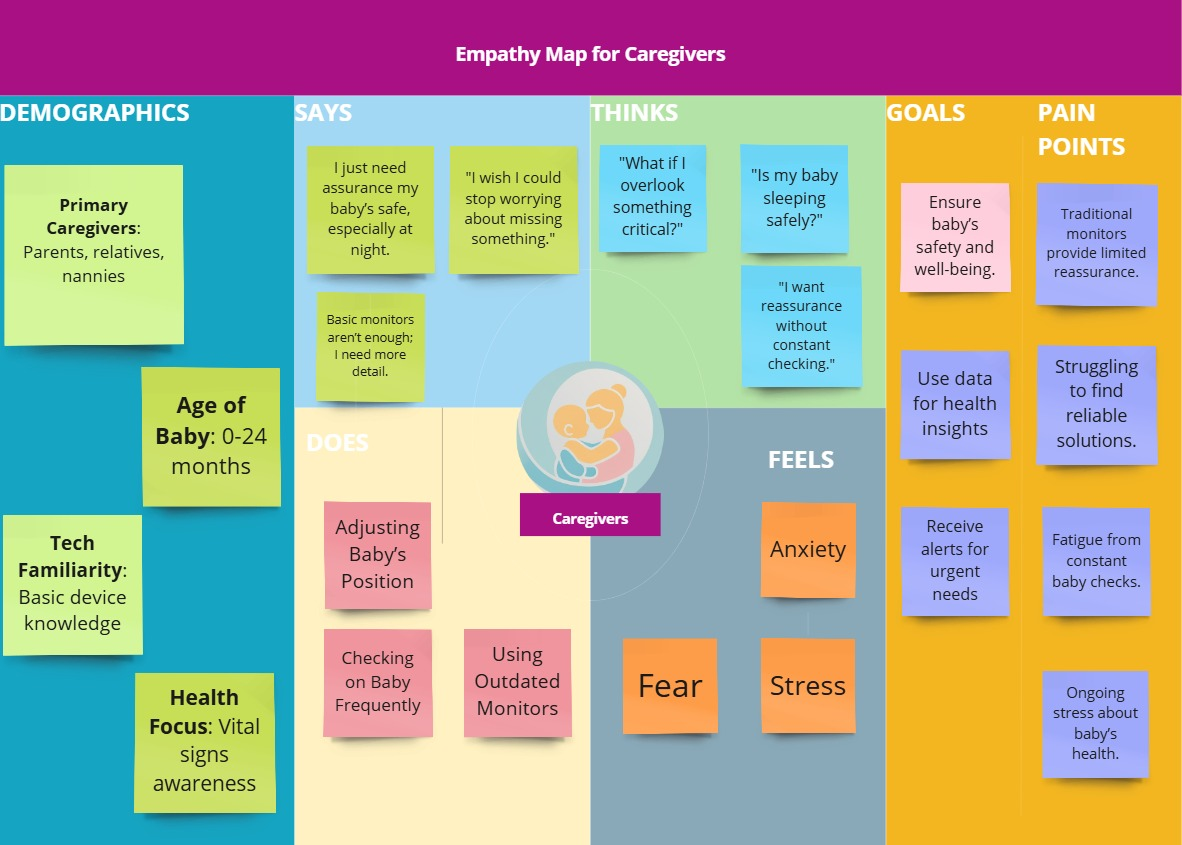
\includegraphics[scale=0.39]{./pic/empathy.jpg}
  \caption{Empathy map capturing caregiver insights for the baby monitoring system.}
  \label{fig:empathy}
\end{figure}


\chapter{Definition}
\section{Point of View (POV)}
Our primary user is a caregiver who experiences anxiety over their baby's safety, especially during sleep. This user needs a reliable way to monitor their baby’s health and safety remotely, without disturbing the baby or physically checking on them throughout the night. They seek reassurance through real-time data on critical health metrics and timely alerts in case of potential dangers, such as abnormal heart rate, body temperature fluctuations, or risky sleep positions that could lead to suffocation or Sudden Infant Death Syndrome (SIDS).

\section{Problem Statement}
Caregivers lack an effective solution for monitoring key health metrics of their baby while being alerted in real-time about potential safety risks. Traditional monitoring devices provide limited information and often lack advanced safety alerts, resulting in heightened stress and interrupted sleep for caregivers. Therefore, we are developing a comprehensive monitoring system that combines real-time data tracking with automatic alerts to enable caregivers to monitor their baby’s well-being remotely, giving them the peace of mind they need.

\chapter{Ideation}
\section{Brainstorming Process}
Our ideation process began with brainstorming sessions among the project team, informed by user insights and empathy mapping. We used methods like mind mapping and the ``How Might We" (HMW) technique to generate solutions that could meet caregivers' needs. We explored various ideas for tracking and alerting on vital signs, developing intuitive interfaces for ease of use, and integrating remote monitoring capabilities.

In these sessions, we outlined the major components required to meet our problem statement: sensors for capturing body metrics (like temperature and heart rate), a real-time alert system, remote connectivity to allow monitoring from anywhere, and an intuitive dashboard or mobile app interface for caregivers.

\section{Idea Highlights}
The final set of ideas prioritized caregiver needs, focusing on creating a monitoring solution with the following key features:
\begin{enumerate}
  \item \textbf{Non-Invasive Health Monitoring:} Using sensors for continuous tracking of vital metrics without disturbing the baby.
  \item \textbf{Real-Time Alerts:} An alert system to notify caregivers immediately in case of unusual health readings or unsafe sleeping positions.
  \item \textbf{Remote Access via Mobile App:} An easy-to-use mobile app that displays live data, health history, and customization options for alert settings.
  \item \textbf{User-Centered Interface Design:} Simple, intuitive interface allowing quick access to key information without overwhelming caregivers.
\end{enumerate}
These ideas were refined to form the foundation for our prototype, balancing the technical feasibility of each feature with the highest potential for solving caregivers’ core pain points.

\chapter{Prototyping}
\section{Prototype Overview}
Our initial prototype focuses on combining hardware components with a software interface. The hardware includes sensors capable of capturing data on body temperature, heart rate, and baby posture, which is critical for monitoring sleep safety. The mobile app interface allows caregivers to see real-time data on these metrics and customize alert thresholds according to their preferences. We also included a notification system that triggers instant alerts if any health parameter goes outside safe ranges.

We designed the prototype with scalability in mind, ensuring future additions (like more health metrics or connectivity options) could be easily integrated. The prototype is aimed at being user-friendly and accessible, while providing the essential functionalities required for effective baby monitoring.

\section{Images/Samples}
\subsection{Architectural Diagram}
The architectural diagram in Figure \ref{fig:architecture} illustrates the Cloud-Based Smart Monitoring System for Baby Health and Safety, detailing how different components interact to provide comprehensive monitoring.
\begin{itemize}
  \item \textbf{User Interface:} The user starts the monitoring through a mobile app, which includes a live camera feed and displays alerts related to the baby’s health and safety.
  \item \textbf{Sensing System:} Various sensors (heart rate, temperature, $SpO_2$, humidity, noise, and a camera) collect real-time data on the baby’s health and environment. This data is sent to the Processor for preliminary analysis.
  \item \textbf{Processor (Raspberry Pi):} The processor aggregates sensor data and forwards it to the ML Model for posture detection, while also sending processed responses back to the mobile app. It handles computational tasks and initiates alerts if any unsafe conditions are detected.
  \item \textbf{ML Model and Database:} The ML model, hosted externally, analyzes data for unsafe sleeping postures. All sensor and processed data are stored in Firebase, which also triggers alerts and allows historical data retrieval.
  \item \textbf{Alerts:} The system generates alerts when abnormal health metrics or unsafe postures are detected, notifying the user through the app.
\end{itemize}
This streamlined architecture ensures efficient data collection, analysis, and timely alerts, providing a reliable system for monitoring baby health and safety.
\begin{figure}[hbtp]
  \centering
  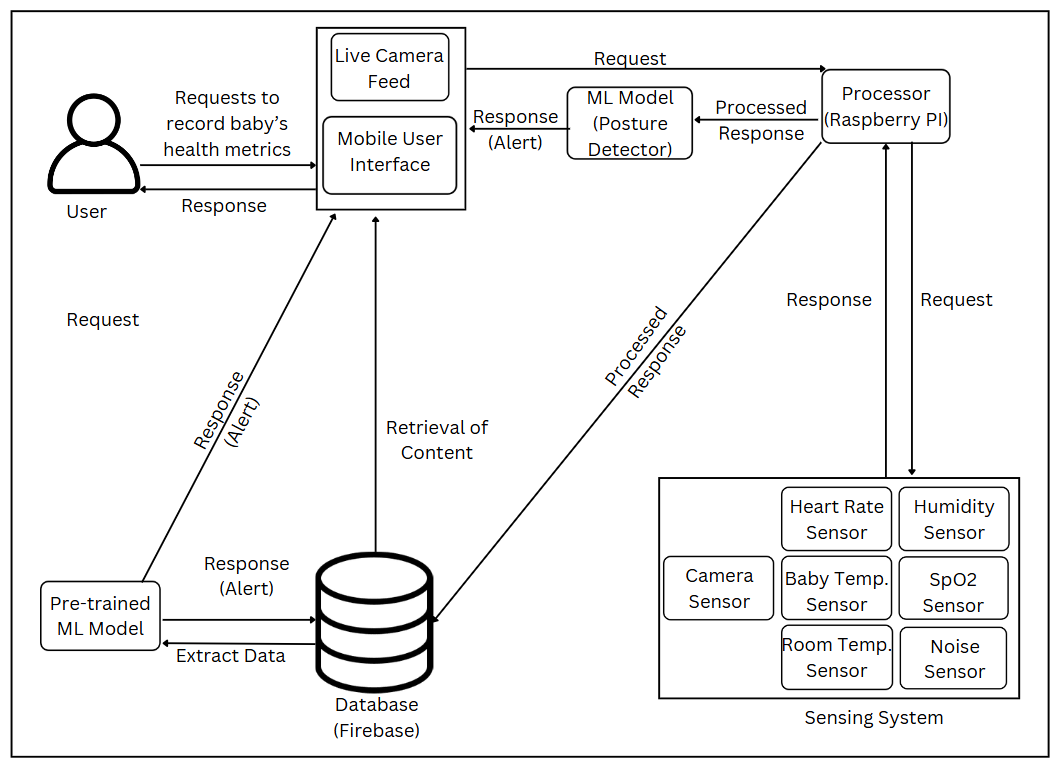
\includegraphics[scale=0.58]{./pic/finarch.png}
  \caption{Architectural Diagram illustrating interactions within the baby monitoring system.}
  \label{fig:architecture}
\end{figure}

\subsection{Use Case Diagram}
The use case diagram in Figure \ref{fig:usecase} illustrates interactions between the caregiver and the baby monitoring system, emphasizing key functionalities.

\begin{itemize}
  \item \textbf{Actors:}
        \begin{itemize}
          \item \textbf{Primary Actor:} Parents or caregivers who rely on the mobile app for real-time data and notifications about the baby's status.
          \item \textbf{Secondary Actors:} Medical professionals or support staff who may access the system during emergencies.
        \end{itemize}

  \item \textbf{Use Cases:}
        \begin{itemize}
          \item \textbf{Monitoring Baby’s Health Metrics:} Displays real-time information (temperature, heart rate, humidity, $SpO_2$) on the dashboard for continuous monitoring.
          \item \textbf{Viewing Live Video Feeds:} Allows caregivers to access live video streams of the baby’s crib or play area for constant visual monitoring.
          \item \textbf{Receiving Alerts for Abnormal Conditions:} Sends instant notifications for unsafe conditions (e.g., rolling over, abnormal heart rate, high temperature).
          \item \textbf{Managing System Settings:} Enables configuration of thresholds, notification preferences, and video quality, as well as toggling between real-time and historical views.
          \item \textbf{Exporting Historical Data:} Allows Parents to view or export historical health data for further analysis or sharing with healthcare professionals.
        \end{itemize}
\end{itemize}

\begin{figure}[hbtp]
  \centering
  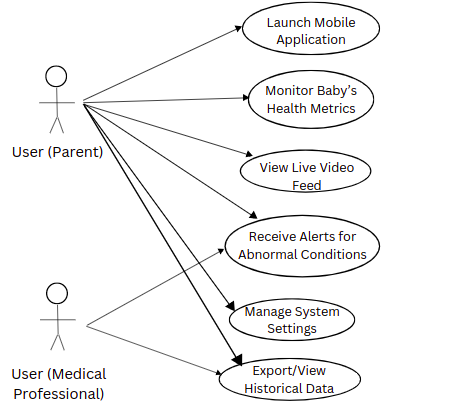
\includegraphics[scale=0.6]{./pic/usercase.png}
  \caption{Use Case Diagram illustrating interactions between users and the system.}
  \label{fig:usecase}
\end{figure}

\subsection{Sequence Diagram}
The sequence diagram in Figure \ref{fig:sequence} illustrates the workflow of a Cloud-Based Smart Monitoring System for Baby Health and Safety. Here’s a breakdown of the interactions among various components in the system:

\begin{enumerate}
  \item \textbf{User Interaction and Mobile Application:} The user opens the mobile app to start monitoring the baby’s health. Through the app, they initiate requests to fetch various health metrics like heart rate, humidity, temperatures (body and room), $SpO_2$, and a live video feed. The app interface also displays alerts for abnormal readings.
  \item \textbf{Sensing System:} The sensing system gathers data from different sensors, such as heart rate, room and body temperature, humidity, $SpO_2$, and a camera feed. This collected data is then sent to the Processor for further processing and analysis.
  \item \textbf{ML Model:} After receiving the sensed data, the Processor forwards relevant information to the ML model, which is responsible for posture detection and analyzing the baby’s sleeping position. This step helps in identifying any unsafe sleeping postures.
  \item \textbf{Database:} The processed data, including any abnormal readings or posture alerts, is stored in the database for historical tracking. The database also supports the mobile app by providing stored readings whenever the user requests history.
  \item \textbf{Alerts and Notifications:} If the system detects unsafe postures or abnormal health readings, an alert is triggered and sent back to the mobile app. The user is notified in real-time, allowing them to take immediate action if needed.
\end{enumerate}
This sequence diagram effectively demonstrates how the system monitors and processes vital information, triggering alerts when necessary to ensure the baby’s safety. 
\begin{figure}[hbtp]
  \centering
  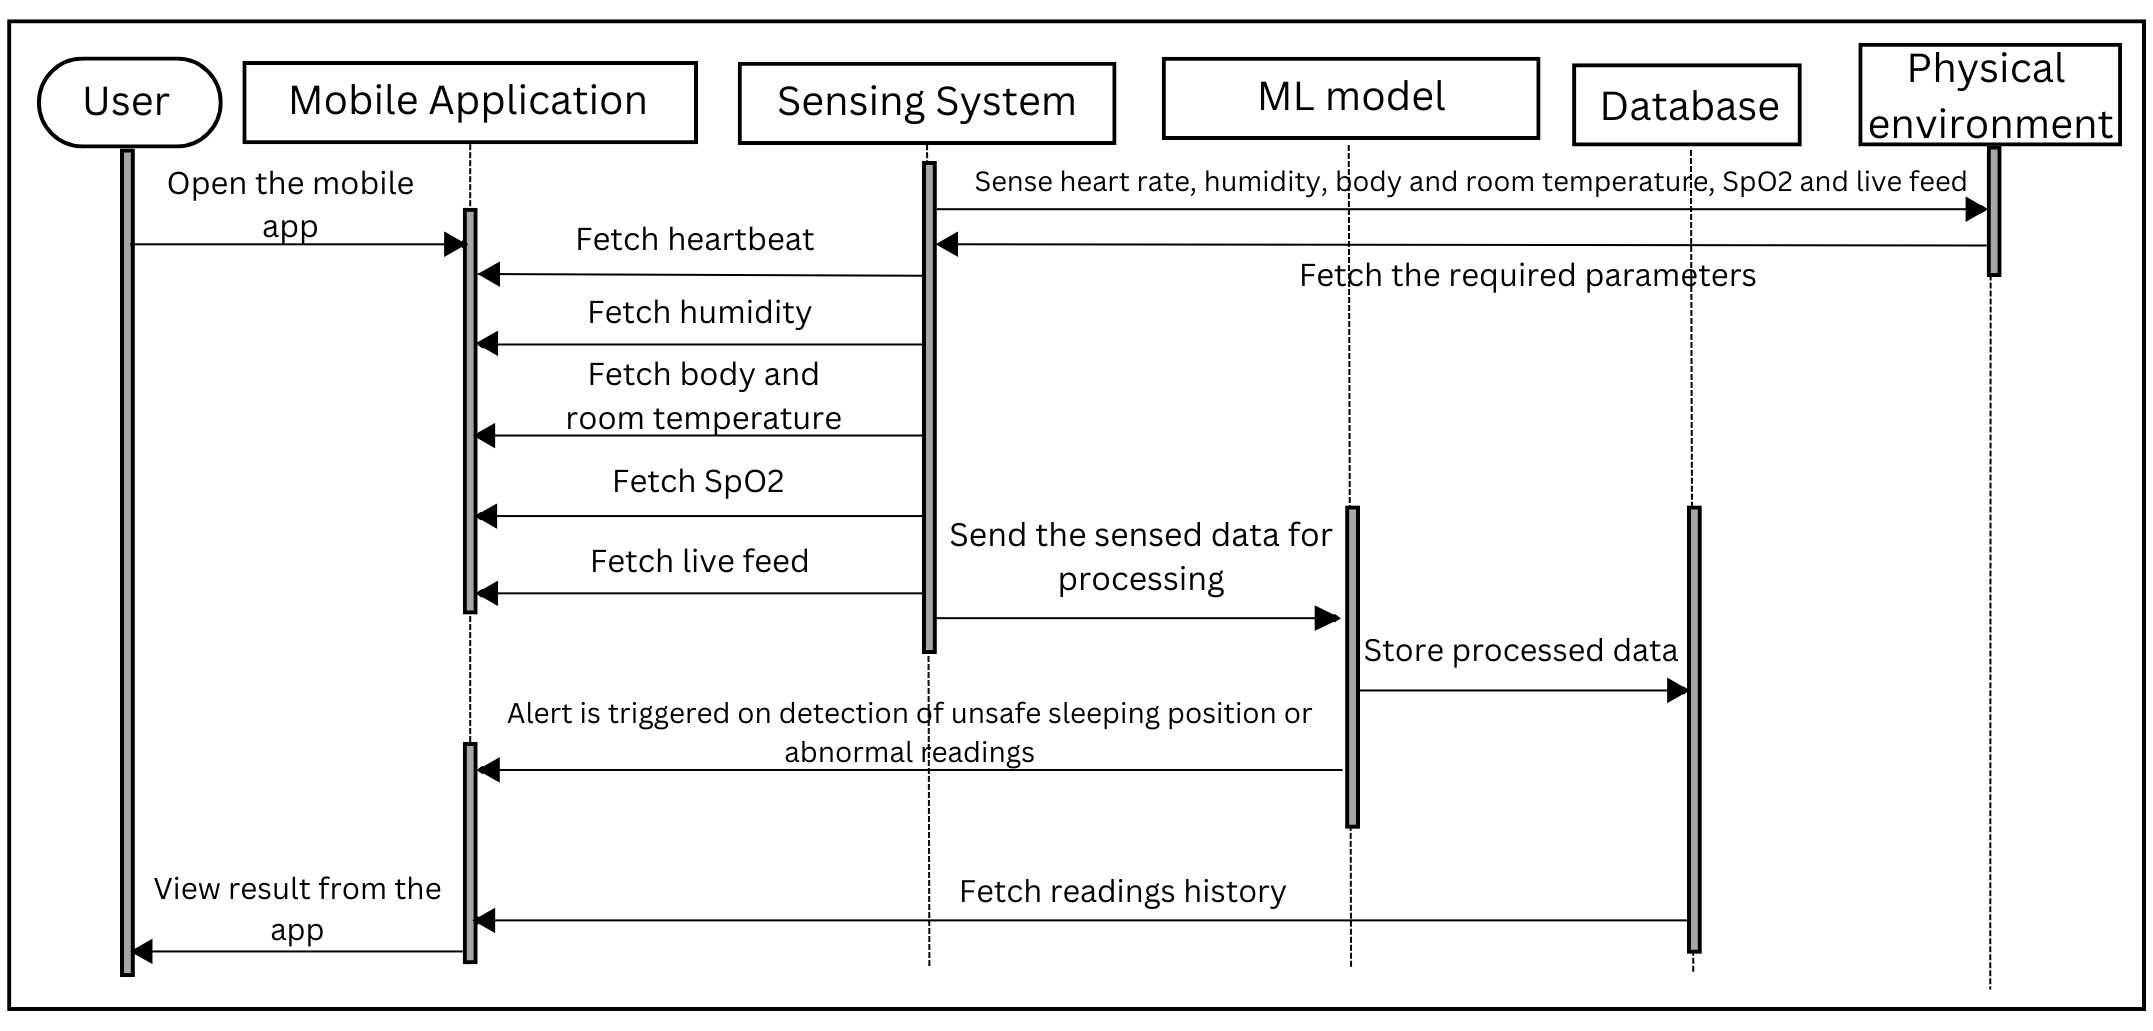
\includegraphics[scale=0.285]{./pic/seq.png}
  \caption{Sequence diagram showing the timeline of interaction between different entities in the system.}
  \label{fig:sequence}
\end{figure}


\subsection{Data Flow Diagram}
The data flow diagram shown in Figure \ref{fig:dataflow} outlines how data travels through the system, highlighting the interaction between sensors, the Raspberry Pi, cloud storage, and the mobile application.

\begin{itemize}
  \item \textbf{Sensors:} IoT sensors collect real-time data on the baby’s health and environmental conditions.
  \item \textbf{Raspberry Pi:} Acts as a bridge, processing sensor data and relaying it to the cloud.
  \item \textbf{Cloud Database:} Data is securely stored and processed in the cloud. The system checks data against safety thresholds and sends alerts for any abnormalities detected.
  \item \textbf{Mobile Application:} The app fetches data from the cloud and displays it to the user in real-time. Parents can also access historical data for deeper insights into the baby’s health trends.
\end{itemize}

\begin{figure}[hbtp]
  \centering
  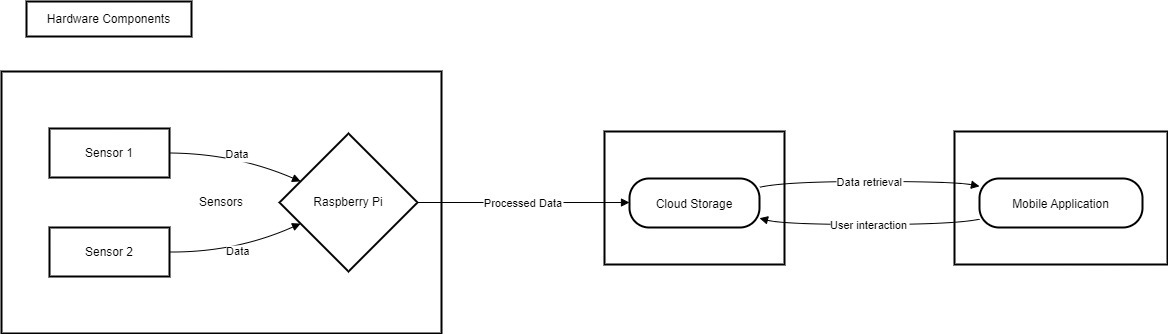
\includegraphics[scale=0.35]{./pic/WhatsApp Image 2024-10-23 at 22.00.55_66baa9c8.jpg}
  \caption{Data flow diagram showing how the data travels through the system.}
  \label{fig:dataflow}
\end{figure}
\subsection{Hardware Components}
The hardware components and their placement in the cradle are shown in Figure \ref{fig:hardware} and Figure \ref{fig:cradle} respectively.

Hardware components that are used are as follows:
\begin{itemize}
  \item \textbf{Raspberry Pi (Model 3B or higher):} Serves as the main processing unit for handling video feeds and interfacing with IoT sensors. It is equipped with a compatible camera module for video input.

  \item \textbf{Camera Module:} A Raspberry Pi camera module will be used for live monitoring, providing real-time video feeds of the baby’s environment.

  \item \textbf{Sensors:}
        \begin{itemize}
          \item \textbf{Temperature Sensor:} DHT22 sensor for accurate temperature measurements.
          \item \textbf{Humidity Sensor:} Monitors ambient humidity levels to ensure a comfortable environment.
          \item \textbf{Heart Rate Sensor:} MAX30100 sensor for measuring the baby's heart rate.
          \item \textbf{$SpO_2$ Sensor:} Monitors blood oxygen saturation levels to track the baby's health.
        \end{itemize}
\end{itemize}

\begin{figure}[H]
  \centering
  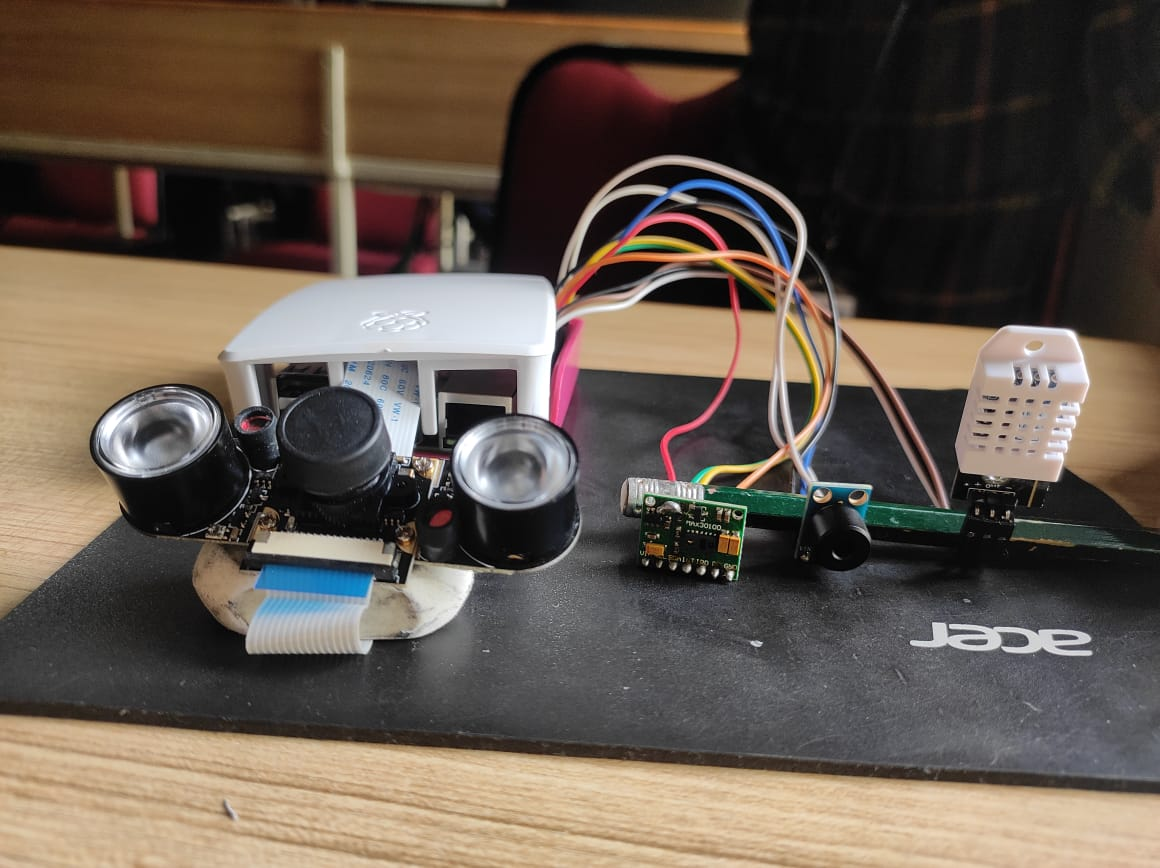
\includegraphics[scale=0.35]{./pic/hardware.jpeg}
  \caption{Hardware components used in the baby monitoring system.}
  \label{fig:hardware}
\end{figure}
\begin{figure}[H]
  \centering
  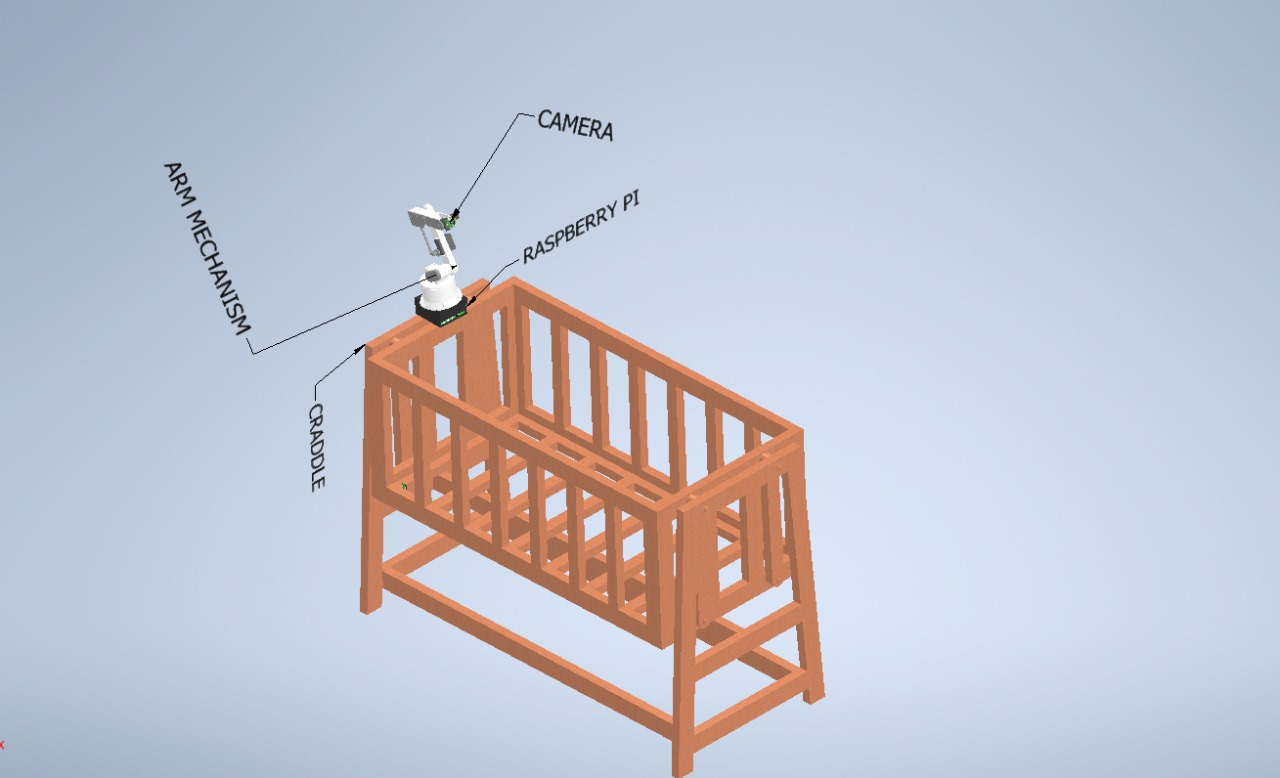
\includegraphics[scale=0.4]{./pic/cradle.jpeg}
  \caption{Placement of the hardware setup in the cradle}
  \label{fig:cradle}
\end{figure}


\chapter{Testing and Feedback}
\section{Testing Process}
To assess the usability and effectiveness of our prototype, we conducted user testing sessions with caregivers who frequently use baby monitoring devices. We simulated various health scenarios (e.g., elevated body temperature, changes in sleep posture) to observe how the prototype detected and reported these events. Users interacted with both the hardware and software components, receiving notifications on a mobile device when specific thresholds were met. The prototype’s alert system and user interface were rigorously tested for clarity, accessibility, and speed in real-time notifications.

\section{Feedback Summary}
Key feedback from caregivers centered around the intuitiveness of the app and the alert functionality. Users appreciated the real-time nature of the notifications, which provided peace of mind. However, some users suggested improvements in customizing the alert sensitivity and simplifying the interface for quicker navigation. Users also recommended adding a “silent mode” for notifications to prevent disturbing other household members during the night. Based on this feedback, we refined the prototype by adding additional alert customization options, simplified app navigation, and included silent alert options, enhancing the overall user experience.

\chapter{Final Solution}
\section{Solution Description}
Our final solution, the Cloud-Based Smart Monitoring System for Baby Health and Safety, is a comprehensive monitoring platform designed to track vital infant health metrics. The system includes a mobile app that interfaces with hardware sensors to continuously monitor body temperature, heart rate, and sleep posture. When irregular readings are detected, caregivers are notified in real-time, allowing them to respond quickly to potential health risks. The platform leverages non-invasive sensor technology to ensure that the monitoring process is comfortable for the baby, while the mobile app interface provides caregivers with an intuitive dashboard for viewing data and adjusting alert settings.

\section{Features}
\begin{enumerate}
  \item \textbf{Real-Time Health Tracking:} Continuous monitoring of critical health metrics such as heart rate, body temperature, and sleep posture.
  \item \textbf{Instant Alerts:} Immediate notifications sent to caregivers if any health metric exceeds predefined safe ranges.
  \item \textbf{Remote Access:} Caregivers can monitor health data and receive alerts through a mobile app from anywhere.
  \item \textbf{Customizable Notifications:} Alert sensitivity and notification settings can be customized to suit caregivers' preferences.
  \item \textbf{Silent Mode:} Notifications can be muted during specific hours, ensuring that other household members are not disturbed.
\end{enumerate}

\section{Visuals}
\subsection{User Interface Flow}
The user interface flow for the application (Figure \ref{fig:uiflow}) is designed to provide Parents with an intuitive and seamless experience for monitoring their baby's health and environment. The following steps describe the flow from the onboarding process to the profile management:
\begin{enumerate}
  \item \textbf{Onboarding Screen:} Upon launching the app, the user is welcomed with the onboarding screen, which introduces the app’s primary function, ensuring peace of mind for every Parent by offering baby health monitoring in the palm of their hand. This screen includes an image carousel showcasing key features like monitoring baby movements, temperature, humidity, and more. The user is prompted to continue with email to proceed further.
  \item \textbf{Sign-Up Screen:} New users are taken to the Sign-Up screen after the onboarding. Here, they can create an account by providing a username, email, and password. A simple and user-friendly form guides the registration process. After filling in the details, they can tap Sign Up. If they already have an account, they are given the option to switch to the login screen.
  \item \textbf{Login Screen:} Existing users access the Login screen, where they can sign in by entering their email and password. There’s also a Forgot password option for those who might need help recovering their credentials. After entering valid credentials, the user taps Log In to access the app’s features.
  \item \textbf{Home Screen:} After logging in, the user is taken to the Home screen. This screen displays key baby health data, including real-time temperature tracking, humidity levels and $SpO_2$ levels.
  \item \textbf{Stats Screen:} The Stats screen gives a detailed view of the baby’s health trends over time.
  \item \textbf{Profile Screen:} The Profile screen offers personalized features for the user. They can call a doctor directly from the app if any issues are detected, access emergency contacts quickly for immediate assistance, modify details such as contact information, health preferences, and other personal settings to ensure the app is tailored to their needs.
\end{enumerate}
\begin{figure}[H]
  \centering
  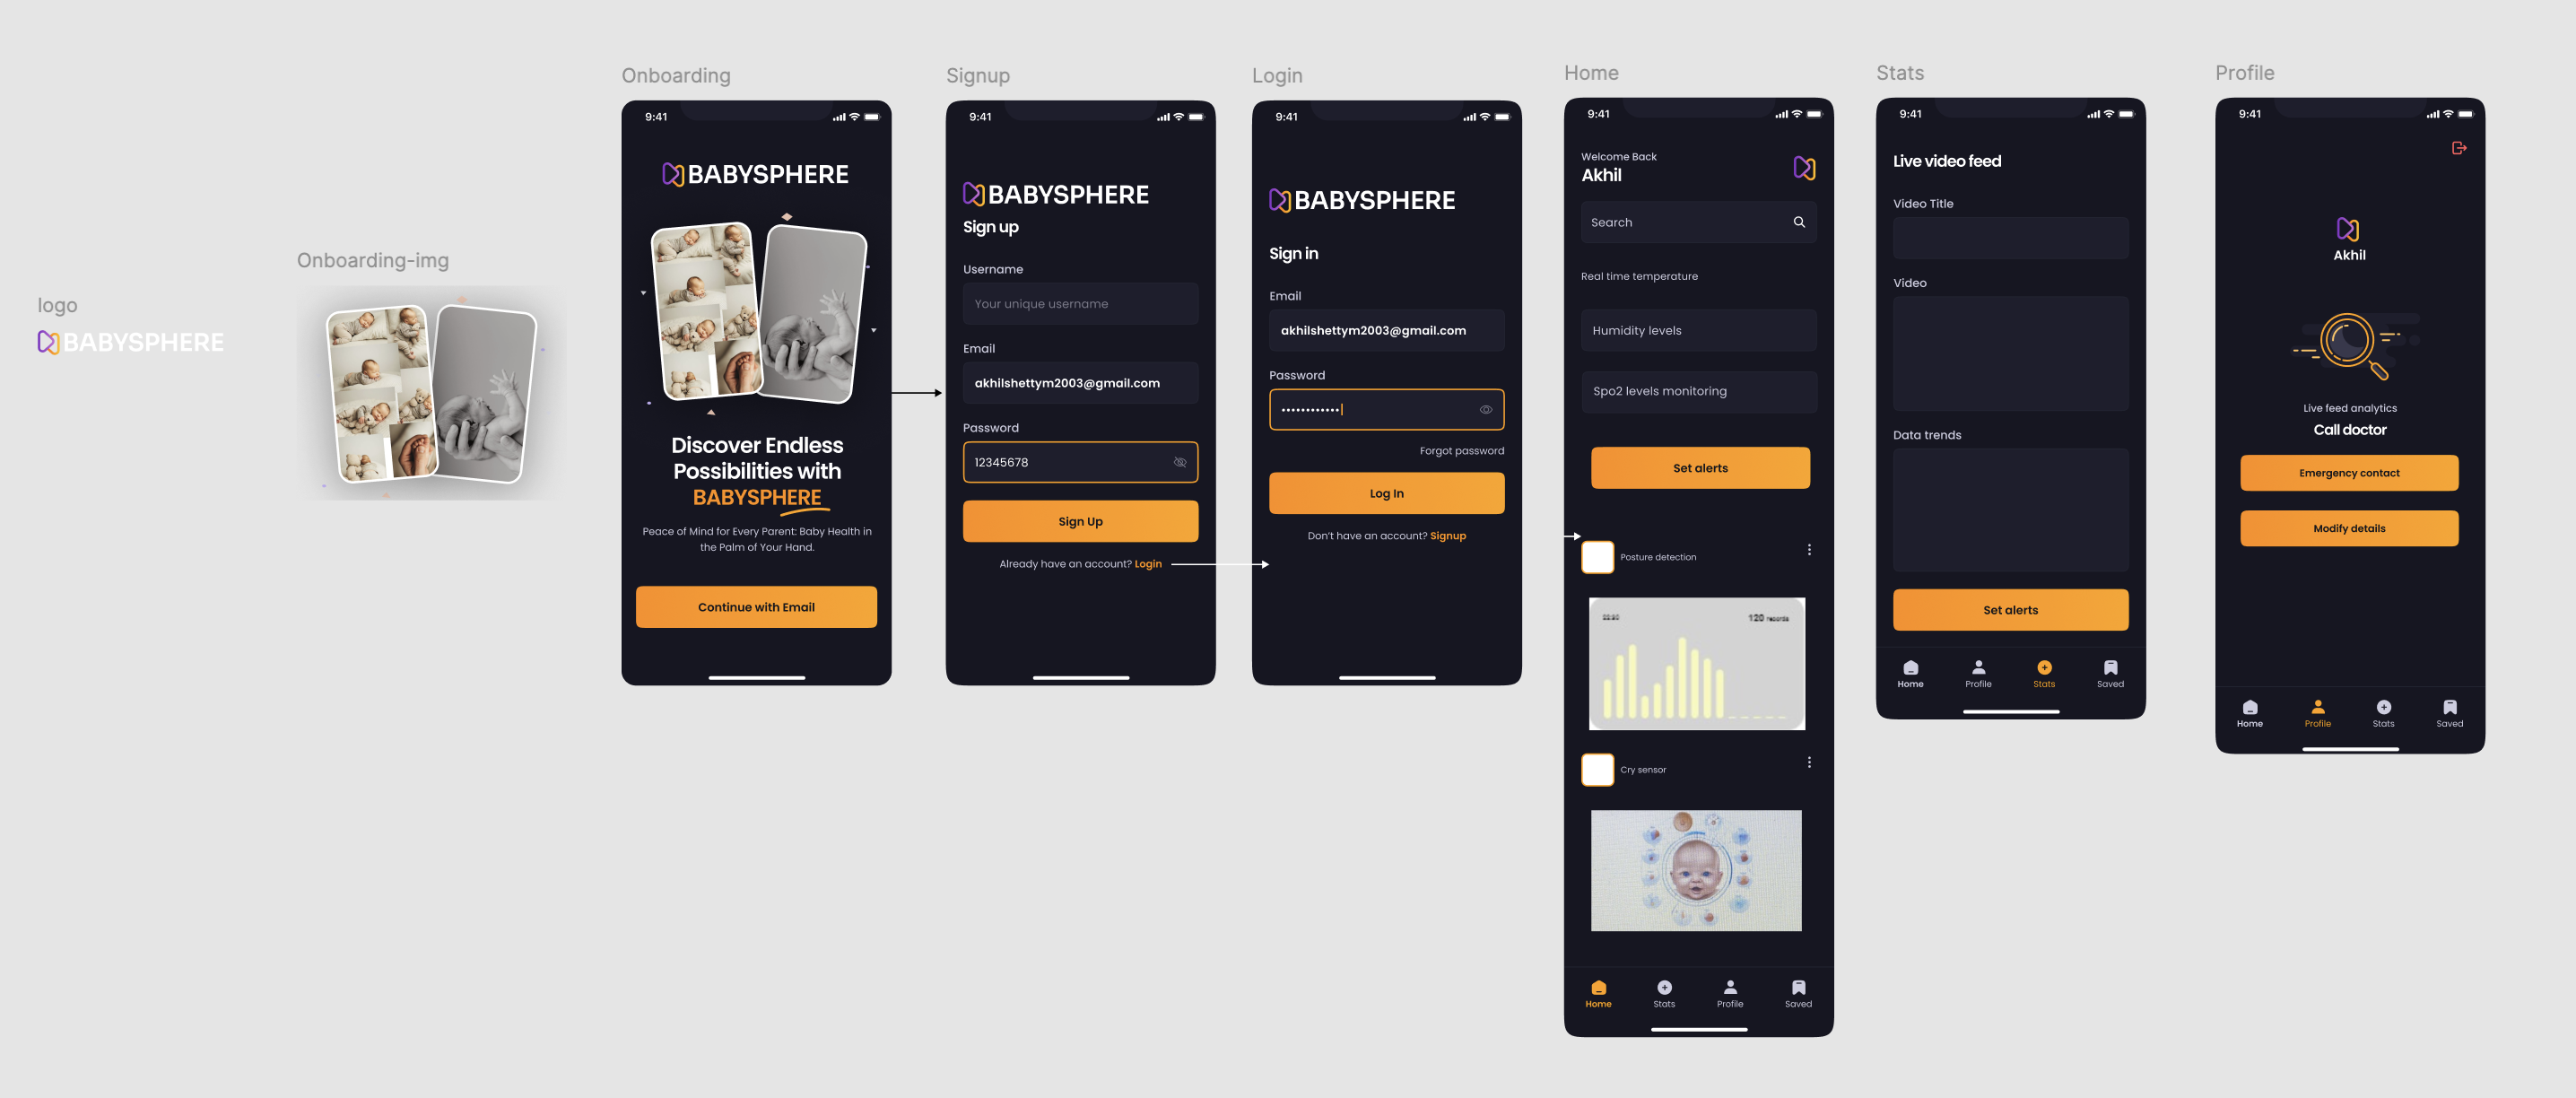
\includegraphics[scale=0.32]{./pic/uiflow.png}
  \caption{User Interface Flow}
  \label{fig:uiflow}
\end{figure}

\chapter{Reflections and Next Steps}
\section{Lessons Learned}
Throughout the project, we gained valuable insights into the importance of iterative testing and user feedback in creating a user-centered product. We learned that caregivers need not only real-time monitoring but also an intuitive interface and customizable alert options to reduce unnecessary notifications. Some technical challenges included balancing the sensitivity of the sensors to avoid false positives while ensuring accuracy in real-life situations. Our team also learned the importance of interdisciplinary collaboration, combining hardware and software skills to develop a fully integrated system.

\section{Future Steps}
To further enhance the solution, we plan to:
\begin{enumerate}
  \item \textbf{Expand Health Metrics: }Include additional metrics such as oxygen saturation and respiratory rate for more comprehensive monitoring.
  \item \textbf{Integrate AI-Based Analysis:} Incorporate machine learning to improve alert accuracy by identifying patterns in baby health data over time.
  \item \textbf{Enhanced Customization Options:} Allow caregivers to create detailed, individualized profiles for different sleep scenarios.
  \item \textbf{Scalability:} Scale the system for use in neonatal intensive care units (NICUs) to help healthcare professionals monitor newborns in hospital settings.
  \item \textbf{Secure Cloud Storage:} Implement encrypted cloud storage for securely storing health data, enabling easy sharing with healthcare providers.
\end{enumerate}

By implementing these next steps, we aim to improve our monitoring system’s functionality, broaden its applications, and continue advancing caregiver support for baby health and safety.

\chapter{Mentor Interactions}
\section{Mentor Role}
Our project mentor played a crucial role in shaping and guiding the direction of the Cloud-Based Smart Monitoring System for Baby Health and Safety. From the initial project selection stage, the mentor provided insights into the relevance of baby health monitoring systems, particularly the gaps in existing solutions regarding real-time alerts and comprehensive health metric tracking. They emphasized the need for a user-centered approach, ensuring that each feature of our project directly addresses a caregiver’s primary concerns and usability needs. The mentor also encouraged us to consider sustainable design elements and scalability, which helped in aligning our project with long-term user expectations and potential growth.

\section{Mentor Value Addition}
Throughout the development process, our mentor provided invaluable feedback on the prototype, offering technical and practical insights that significantly enhanced our solution. During the prototyping phase, the mentor suggested refining the alert system to allow caregivers to customize notification preferences, making the device more adaptable to different caregiving scenarios.

Additionally, our mentor recommended conducting iterative testing with real users early on to identify usability challenges. This advice was instrumental in uncovering interface elements that could be streamlined, such as simplifying the app’s navigation and making the alert dashboard more visually intuitive. Their emphasis on creating a modular design also guided us in structuring the codebase to facilitate future expansion, aligning with our goal of potentially integrating more advanced health metrics.

The mentor’s constructive feedback and continuous support throughout each phase of our project greatly contributed to refining our prototype and building a solution that is both practical and aligned with user needs. Their guidance not only helped us address current challenges but also prepared us to think proactively about future developments and scalability.

\newpage
\renewcommand{\bibname}{References}

\addcontentsline{toc}{chapter}{References}

\printbibliography

\end{document}